% reset section counter
%\setcounter{section}{0}

%\metadata{lecture ID}{Your names}{date}
\metadata{6}{Daniel Do}{February 1st, 2021}

In this chapter, we will instantiate Rademacher complexity for two important hypothesis classes: linear models and two-layer neural networks. In the process, we will develop margin theory and use it to bound the generalization gap for binary classifiers.

\sec{Margin theory for classification problems}

\subsec{Intuition}
Assume that we are in the same setting as in the previous section. A fundamental problem we face in this setting is that we do not have a continuous loss: everything is discrete in the output space. We need to find a way to reason about the scale of the output. An example of this is logistic regression: the logistic regression model outputs a probability, and while we compare it to the outcome (0 or 1), how close it is to the true output gives us a measure of how confident we are in the prediction.

Figure \ref{lec6:fig:margin} gives similar intuition for linear classifiers. Intuitively, the black line is a "better" decision boundary than the red line because the minimum distance from any point to the black boundary is greater than the minimum distance from any point to the red line. In the next section, we will formalize this intuition by proving that the larger this margin is, the smaller the bound on generalization gap is.

\begin{figure}[ht!]
    \begin{center}
  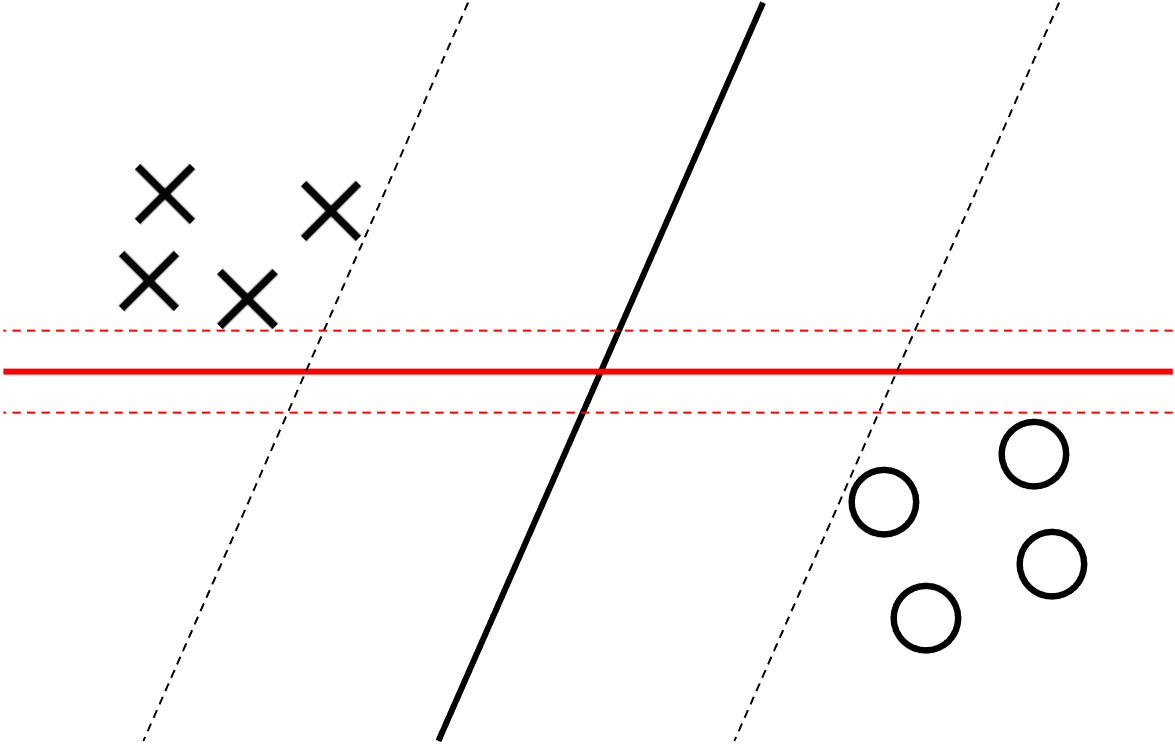
\includegraphics[width=0.5\textwidth]{figures/margin.png}
  \end{center}
  \caption{The red and black lines are two decision boundaries. The X's are positive examples and the O's are negative examples. The black line has a larger margin than the red line, and is intuitively a better classifier.}
  \label{lec6:fig:margin}
\end{figure}

\subsec{Formalizing margin theory}
First, assume that the dataset $\cD = ((x\sp{1}, y\sp{1}), \dots, (x\sp{n}, y\sp{n}))$ is \textit{completely separable}. In other words, there exists some $h_\theta\in\cH$ such that $y^{(i)} = \sgn(h_\theta(x^{(i)}))$ holds for all $( x^{(i)},y^{(i)})\in \cD$. This is not a necessary condition for our final bound but will make the derivation cleaner.

\begin{definition}[(Unnormalized) Margin]
Fix the hypothesis $h_\theta$. The \textit{(unnormalized) margin} for example $(x, y)$ is defined as $\margin(x) = yh_\theta(x)$. Margin is only defined on examples where $\sgn(h_\theta(x)) = y$. (Note that $\margin(x)\geq 0$ because of our assumption of complete separability.)
\end{definition}

\begin{definition}[Minimum margin] Given a dataset $\cD = ((x\sp{1}, y\sp{1}), \dots, (x\sp{n}, y\sp{n}))$, the \textit{minimum margin} over the dataset is defined as $\gamma_{\min} \triangleq \min_{i\in\{1,\dots,|\cD|\}} y^{(i)}h_\theta(x^{(i)})$.
\end{definition}

Our final bound will have the form (generalization gap)$\leq f(\text{margin},\text{parameter norm})$. This is very generic since there are many different bounds we could derive based on what margin we use. For this current setting we are using $\gamma_{\min}$, which is the minimum margin, but in other settings could use $\gamma_{\text{average}}$, which is the average margin of each point in the dataset.

We will begin by introducing the idea of a \textit{surrogate loss}, a loss function which approximates zero-one loss but takes the scale of the margin into account. The \textit{margin loss} (also known as \textit{ramp loss}) is defined as 
\begin{equation}
    \ell_\gamma(t) = \begin{cases} 
      0 & t\geq \gamma \\
      1 & t\leq 0 \\
      1-t/\gamma & 0\leq t\leq \gamma
   \end{cases}
\end{equation}

\begin{figure}[ht!]
    \begin{center}
  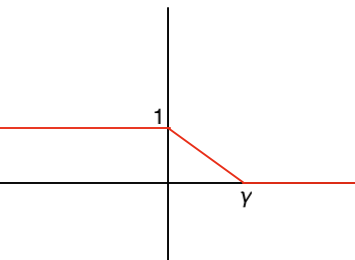
\includegraphics[width=0.5\textwidth]{figures/margin_loss.png}
  \end{center}
  \caption{Plotted margin loss.}
  \label{lec6:fig:marginloss}
\end{figure}

It is plotted in Figure \ref{lec6:fig:marginloss}. For convenience, define $\ell_\gamma((x,y), h) \triangleq \ell_\gamma(yh(x))$. We can view $\ell_\gamma$ as a continuous version of $\err$ while being more sensitive to the scale of the margin on $[0,\gamma]$. Notice that $\err$ is always less than or equal to the $\ell_\gamma$ when $\gamma\geq 0$, i.e.
\begin{equation}
    \err((x,y), h) = \ind{yh(x) < 0}\leq \ell_\gamma(yh(x)) =\ell_\gamma ((x,y), h)
\end{equation}
holds for all $(x,y)\sim P$. Taking the expectation over $(x,y)$ on both sides of this inequality, we see that
\begin{equation}
    L(h) = \E_{(x,y)\sim P} \left[ \err((x,y), h) \right] \leq \E_{(x,y)\sim P} \left[ \ell_\gamma ((x,y), h) \right].
\end{equation}

Therefore, the population loss is bounded by the expectation of the margin loss, and so it is sufficient to bound the expectation of the margin loss in order to bound the population loss.

Define the population and empirical version of the margin loss:
\begin{equation}
L_\gamma(h) = \E_{(x,y)\sim P}\l[ \ell_\gamma((x,y), h)\r], \quad \hat{L}_\gamma(h) = \sum_{i=1}^n\l [\ell_\gamma((x^{(i)},y^{(i)}), h)\r].
\end{equation}

By Corollary \ref{lec6:cor:ggap-rsbound}, we see that with probability at least $1-\delta$ that
\begin{equation}
L_\gamma(h) - \hat{L}_\gamma(h)\leq 2R_S(\cF) + 3\sqrt{\frac{\log (2/\delta)}{2n}},
\end{equation}
where $\cF = \{(x,y)\mapsto \ell_\gamma((x,y), h)\mid h\in\cH\}$. Note that if we set $\gamma\leq \gamma_{\min}$, then $\hat{L}_{\gamma}(h) = 0$. This follows because by definition of $\gamma_{\min}$, $y^{(i)}h(x^{(i)})\geq \gamma_{\min}$ for any $(x^{(i)}, y^{(i)})\in \cD$. As a result, $\ell_\gamma((x^{(i)}, y^{(i)}), h) = \ell_\gamma(y^{(i)}h(x^{(i)})) = 0$ holds. Therefore, it suffices to bound $R_S(\cF)$.

We will now use \textit{Talagrand's lemma} to bound $R_S(\cF)$ in terms of $R_S(\cH)$ to remove any dependence on the loss function from the upper bound. 
 
\begin{lemma}{(Talagrand's lemma)}
Let $\phi:\R\to\R$ be a $\kappa$-Lipschitz function. Then \begin{equation}
    R_S(\phi\circ \cH)\leq \kappa R_S(\cH),
\end{equation} 
where $\phi\circ\cH = \{z\mapsto \phi(h(z))\mid h\in\cH\}$.
\end{lemma}

We can use Talagrand's lemma directly with $\phi(t) = \ell_\gamma(t)$, which is $\frac{1}{\gamma}$-Lipschitz. We can express $\cF$ as $\cF=\ell_\gamma\circ\cH'$ where $\cH' = \{(x,y)\to yh(x)\mid h\in\cH\}$. Applying Talagrand's lemma, we see that

\begin{align}
R_S(\cF) &\leq \frac{1}{\gamma}R_S(\cH') \\
&= \frac{1}{\gamma}\E_{\sigma_1,\dots, \sigma_n} \l[ \sup_{h\in \cH} \frac{1}{n} \sum^n_{i=1} \sigma_i y^{(i)}h(x^{(i)}) \r] \\
&= \frac{1}{\gamma}\E_{\sigma_1,\dots, \sigma_n} \l[ \sup_{h\in \cH} \frac{1}{n} \sum^n_{i=1} \sigma_i h(x^{(i)})  \r] \\
&= \frac{1}{\gamma}R_S(\cH).
\end{align}

Putting this all together, we have shown that for $\gamma = \gamma_{\min}$,
\begin{align}
\Err(h) \leq L_\gamma(h) &\leq 0 + O \left( \frac{R_S(\cH)}{\gamma} \right) + \tilO \left( \sqrt{\frac{\log (2 / \delta)}{2n}} \right) \\
&= O \left( \frac{R_S(\cH)}{\min_i y\sp{i} h(x\sp{i}) } \right) + \tilO \left( \sqrt{\frac{\log (2 / \delta)}{2n}} \right).
\end{align}

In other words, for training data of the form $S = \{(x\sp{i},y\sp{i})\}_{i=1}^n \subset \mathbb{R}^d \times \{-1,1\}$, a hypothesis class~$\mathcal{H}$ and 0-1 loss, we can derive a bound of the form
\begin{equation}\label{lec7:eqn:generalization_loss}
    \text{generalization loss} \leq \frac{2R_S(\mathcal{H})}{\gamma_{\mathrm{min}}} + \text{low-order term},
\end{equation}
where $\gamma_\mathrm{min}$ is the minimum margin achievable on~$S$ over those hypotheses in $\cH$ that separate the data, and $R_S(\cH)$ is the empirical Rademacher complexity of $\cH$. Such bounds state that simpler models will generalize better beyond the training data, particularly for data that is strongly separable.

\begin{remark}
Note there is a subtlety here. If we think of the dataset as random, it follows that $\gamma_{\min}$ is a random variable. Consequently, the $\gamma$ we choose to define the hypothesis class is random, which is not a valid choice when thinking about Rademacher complexity! Technically we cannot apply Talagrand's lemma with a random $\kappa$ (which we took to be $1/\gamma$). Also, when we used concentration inequalities, we implicitly assume that the $\ell_\gamma((x\sp{i}, y\sp{i}), h)$ are independent of each other. That is not the case if $\gamma$ is dependent on the data.

We sketch out how one might address this issue below. The main idea is to do another union bound over $\gamma$. Choose a family $\Gamma = \left\{ 2^k: k \in [-B, B] \right\}$ for some $B$. Then, for every fixed $\gamma \in \Gamma$, with probability greater than $1 - \delta$,
\begin{align}
\Err(h) \leq \hatL_\gamma (h) + O \left( \frac{R_S(\cH)}{\gamma} \right) + \tilO \left( \sqrt{\frac{\log \frac{1}{\delta}}{n}} \right).
\end{align}
Taking a union bound over all $\gamma \in \Gamma$, it further holds that for all $\gamma \in (0, B)$, 
\begin{align}
    \Err(h) \leq \hatL_\gamma (h) + O \left( \frac{R_S(\cH)}{\gamma} \right) + \tilO \left( \sqrt{\frac{\log \frac{1}{\delta}}{n}}\right) + \tilO \left ( \sqrt{\frac{\log B}{n}} \right ). \label{lec7:eqn:unionboundmargin}
\end{align}
Last, choose the largest $\gamma \in \Gamma$ such that $\gamma \leq \gamma_{\min}$. Then, for this value of $\gamma$, our desired bound directly follows from the bound in \eqref{lec7:eqn:unionboundmargin}. Namely, we have that $\hatL_{\gamma} (h) = 0$ and $O \left( \frac{R_S(\cH)}{\gamma} \right) = O \left( \frac{R_S(\cH)}{\gamma_{\min}} \right)$. The additional term, $\tilO\left ( \sqrt{\frac{\log B}{n} }\right )$, is the price exacted by the uniform convergence argument required to correct the heuristic bound given in \eqref{lec7:eqn:generalization_loss}.

\end{remark}